% \documentclass[draft]{beamer}
\documentclass{beamer}

\usepackage{tikz}
\usepackage{pgf}
\usepackage{amsmath, amssymb, amsthm}
\usepackage{xspace}

\usetheme{Dresden}
\usecolortheme{default}
% \usecolortheme{dolphin}

\newcommand{\el}{\ensuremath{\mathcal{EL}}\xspace}
\newcommand{\alc}{\ensuremath{\mathcal{ALC}}\xspace}
\newcommand{\I}{\ensuremath{\mathcal{I}}\xspace}
\newcommand{\exptime}{\ensuremath{\textsc{ExpTime}}\xspace}
\newcommand{\pspace}{\ensuremath{\textsc{PSpace}}\xspace}

\renewcommand{\emph}[1]{\textcolor{blue}{#1}}
\title{Probabilistic \el}
\author{Jean Christoph Jung}
\date{19.01.2010}
\institute[TdKI Bremen]{AG Theoretische Grundlagen der K\"unstlichen Intelligenz \\ Universit\"at Bremen}

\begin{document}
\begin{frame}
	\titlepage
\end{frame}


\begin{frame}
  \frametitle{Motivation}
  \begin{itemize}
    \item Description Logics are accepted formalism for KR
    \item polynomial time reasoning for \el
    \item desired: ability to represent \emph{uncertain knowledge}
  \end{itemize}

  \emph{Example} 
  \begin{itemize}
%     \item partner of mother is probably the father
    \item a certain indication has a probable cause
    \item a finding is not certain
    \item somebody with a flew has fever with at least $75\%$
  \end{itemize}
\end{frame}


\begin{frame}
  \frametitle{Description Logics}
  \begin{itemize}
    \item family of logics to describe terminological knowledge
    \item decidable fragments of FOL
    \item 
      Concepts:	$C: :=\top~|~A~|~\neg C~|~C_1\sqcap C_2~|~\exists r.C~|~\ldots$
    \item 
      terminological knowledge (TBox): set of GCIs $C\sqsubseteq D$
    \item
      instance knowledge (ABox): set of assertions $C(a)$, $r(a,b)$
  \end{itemize}
  \emph{Example}
  \begin{align*}
    Mother &\sqsubseteq Female\sqcap\exists child.\top \\
    Parent &\equiv Mother\sqcup Father \\
    GrandMother &\sqsubseteq Mother \sqcap\exists child.Parent
  \end{align*}
\end{frame}


\begin{frame}
  \frametitle{Semantics}
  given by interpretations $\I=(\Delta,\cdot^{\I})$
  \begin{itemize}
    \item domain $\Delta$, set of individuals
    \item concept names: $A^{\I}\subseteq\Delta$
    \item conjunction: $(C_1\sqcap C_2)^{\I}=C_1^{\I}\cap C_2^{\I}$
    \item negation: $(\neg C)^{\I}=\Delta\setminus C^{\I}$
    \item roles: $r^{\I}\subseteq\Delta\times\Delta$
    \item existential restrictions: $(\exists r.C)^{\I}=\{d\in\Delta~|~\exists e\in C^{\I}.(d,e)\in r^{\I}\}$
  \end{itemize}
\end{frame}


\begin{frame}
  \frametitle{Reasoning in \el}
  \el: restriction to constructors $\exists r.A$ and $\sqcap$
  \begin{itemize}
    \item turns out to be expressive enough in many cases (\mbox{e.g.} medical knowledge bases)
    \item \emph{polynomial} reasoning
    \item extensions: role hierarchies, fixpoint operators, $\bot$, $\dots$
    \item finite model property 
    \item \emph{convex logic}: $C\sqsubseteq D_1\sqcup D_2$ implies $C\sqsubseteq D_1$ or $C\sqsubseteq D_2$
  \end{itemize}
  important observation: \emph{non-convex} extensions of \el are as hard as the corresponding variant of \alc.
\end{frame}


\begin{frame}
  \frametitle{Semantics for Probabilities}
  \begin{itemize}
    \item important problem in philosophy: mathematical, classical, subjective, frequency, $\ldots$
    \item desired: formal semantics for probabilities
    \item FOL: statistical vs. subjective interpretation \cite{halpern}
    \item probability distribution on the domain vs. \emph{possible world semantics}
  \end{itemize}
\end{frame}


\begin{frame}
  \frametitle{Possible World Semantics}
  \begin{itemize}
    \item additional concept constructors $P_{\geq p}C$, $\exists P_{\geq p}r.C$
    \item extend DL-interpretation with a set of worlds
    \item probability distribution on the worlds % (including 0-worlds)
    \item concept \& role names are interpreted locally: $A^{\I,w}$, $r^{\I,w}$
    \item interpretation of new constructors:
      $$(P_{\geq p}C)^{\I,w}=\{d\in\Delta~|~\sum_{v:d\in C^{\I,v}}Pr(v)\geq p\}$$
      $$(\exists P_{\geq p}C)^{\I,w}=\{d\in\Delta~|~\exists e\in C^{\I,w}.\sum_{v:(d,e)\in r^{\I,v}}Pr(v)\geq p\}$$
  \end{itemize}
\end{frame}

\begin{frame}
  \frametitle{Possible World Semantics -- Example}
  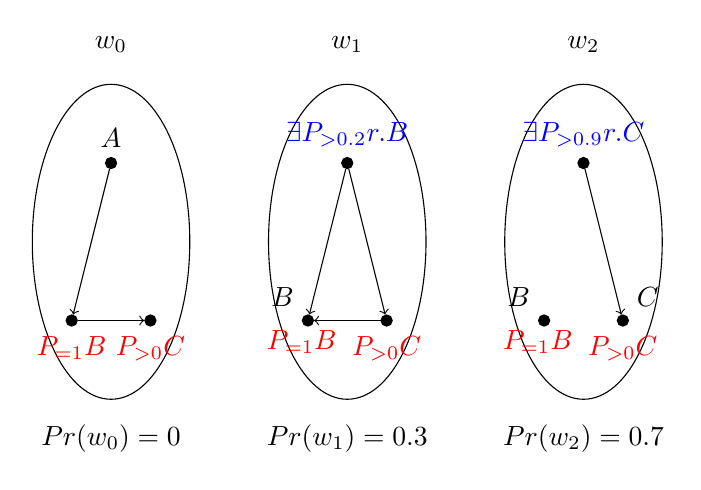
\begin{tikzpicture}[
    indi/.style={
    circle,
    draw=black, 
    fill=black,
    inner sep=.05cm
    }]
    % 		\draw [help lines] (0,0) grid (10, 6);

    \node at (1.5,5.5) {$w_0$};
    \node at (4.5,5.5) {$w_1$};
    \node at (7.5,5.5) {$w_2$};
    \draw (1.5,3) ellipse (1 and 2); 
    \draw (4.5,3) ellipse (1 and 2);
    \draw (7.5,3) ellipse (1 and 2);
    \node[indi,label=above:$A$] at (1.5,4) (a01) {};
    \node[indi] at (1,2) 	 (a02) {};
    \node[indi] at (2,2) 	 (a03) {};
    \node[indi] at (4.5,4) (a11) {};
    \node[indi,label=above left:$B$] at (4,2)   (a12) {};
    \node[indi] at (5,2)   (a13) {};
    \node[indi] at (7.5,4) (a21) {};
    \node[indi,label=above left:$B$] at (7,2) 	 (a22) {};
    \node[indi,label=above right:$C$] at (8,2)   (a23) {};
    \draw[->] (a01) -- (a02);
    \draw[->] (a02) -- (a03);
    \draw[->] (a11) -- (a13);
    \draw[->] (a21) -- (a23);
    \draw[->] (a11) -- (a12);
    \draw[->] (a13) -- (a12);
    \pause
    \node at (1.5, 0.5) {$Pr(w_0)=0$};
    \node at (4.5, 0.5) {$Pr(w_1)=0.3$};
    \node at (7.5, 0.5) {$Pr(w_2)=0.7$};
    \pause
    \node[red, below] at (a02.south) {$P_{=1}B$};
    \node[red, below] at (a03.south) {$P_{>0}C$};
    \pause
    \node[red, below] at (a12.west) {$P_{=1}B$};
    \node[red, below] at (a22.west) {$P_{=1}B$};
    \node[red, below] at (a13.south) {$P_{>0}C$};
    \node[red, below] at (a23.south) {$P_{>0}C$};
    \pause
    \node[blue, above] at (a11.north) {$\exists P_{>0.2} r.B$};
    \pause
    \node[blue, above] at (a21.north) {$\exists P_{>0.9} r.C$};
  \end{tikzpicture}
\end{frame}

\begin{frame}
  \frametitle{Worlds with probability zero}
  \begin{itemize}
    \item takes time getting used to it
    \item philosophical justification: \\
      logically contradictory \emph{$\Longleftrightarrow$} infinitely improbable
    \item special behaviour, since probabilistic operators range only over worlds $w$ with $Pr(w)>0$
    \item often: restriction to one world with probability 0 possible
    \item difference between $\Box C$ and $P_{=1}C$, \mbox{e.g.}, no direct reduction from $S5_{\alc}$
      to Prob-$\alc^{01}$ possible
  \end{itemize}
\end{frame}


\begin{frame}
  \frametitle{Probabilistic \el}
  aims for the design of \emph{``Prob-\el''}:
  \begin{itemize}
    \item add probabilistic constructors
    \item retain polynomial reasoning
  \end{itemize}

%   we show \exptime lower bounds by showing \emph{nonconvexity}
\end{frame}

\begin{frame}
  \frametitle{Attempt 1 -- $P_{>0}C$ and $P_{>0.4}C$}
%   We add the constructors \emph{$P_{>0}C$} and \emph{$P_{>0.4}A$}. 

  Consider the KB $\mathcal K=(\mathcal T, \{C(a)\})$ with $\mathcal T$: 
  \begin{align*}
    C &\equiv P_{>0.4}A_1\sqcap P_{>0.4}A_2\sqcap P_{>0.4}A_3 \\
    D_1 &\equiv P_{>0}(A_1\sqcap A_2) \\
    D_2 &\equiv P_{>0}(A_1\sqcap A_3) \\
    D_3 &\equiv P_{>0}(A_2\sqcap A_3)
  \end{align*}

  \pause
  Now we have $$\mathcal K\models D_1(a)\sqcup D_2(a)\sqcup D_3(a)$$ but for all $i=1,2,3$ $$\mathcal K\not\models D_i(a)$$
\end{frame}


\begin{frame}
  \frametitle{Attempt 2 -- $P_{<1/3}$ and $\bot$}

  Consider TBox: 
  \begin{align*}
    A_1\sqcap A_2 &\sqsubseteq\bot \\
    A_2\sqcap A_3 &\sqsubseteq\bot \\
    A_1\sqcap A_3 &\sqsubseteq\bot
  \end{align*}

  \pause
  We obtain 
  $$\mathcal K\models P_{<1/3}A_1(a)\sqcup P_{<1/3}A_2(a)\sqcup P_{<1/3}A_3(a)$$ but for all $i=1,2,3$ 
  $$\mathcal K\not\models P_{<1/3}A_i(a)$$
\end{frame}

\begin{frame}
  \frametitle{Attempt 3 -- $P_{>p}C$}
  Assume $p=1/k$ for some positive integer $k$.

  Consider now the knowledge base $\mathcal K=(\mathcal T, \mathcal A)$ with

  $$\mathcal T=\{A_i\sqcap A_j\sqsubseteq P_{>p}C_{ij}~|~1\leq i<j\leq k\}$$

  and 

  $$\mathcal A=\{P_{>p}A_i(a)~|~1\leq i\leq k\}$$
  

  \pause
  Then, $$\mathcal K \models \bigsqcup_{i<j}P_{>p}C_{ij}$$
\end{frame}


\begin{frame}
  \frametitle{Result}
  Many interesting combinations of $\el$ with 
  probabilistic operators lead to intractable reasoning. 

  Three possible settings:

  \begin{enumerate}
    \item restriction to ``normal'' TBoxes + $P_{>p}C$ for one probabilty $p$
    \item TBoxes without probabilities, but still only one probability $P_{>p}C$
    \item restriction to $P_{>0}C$ and $P_{=1}C$
  \end{enumerate}
\end{frame}


\begin{frame}
  \frametitle{Probabilities on the roles}
  \begin{itemize}
    \item adding arbitrary $\exists P_{>p}r.C$ leads to similar problems 
    \item So again, try $\exists P_{>0}r.C$ or $\exists P_{=1}r.C$. 
    \item convex extension
    \item From \cite{ls} it is known that \el extended with $P_{>0}C$ and one of the two constructors is \pspace-hard
    \item best known upper bound: 2-$\exptime$.
  \end{itemize}
\end{frame}

\begin{frame}
  \frametitle{The logic $S5_{\el}$}
  \begin{itemize}
    \item two-dimensional logic with possible world semantics
    \item $\Diamond C$ roughly $P_{>0}C$ and $\exists\Diamond r.C$ roughly $\exists P_{>0}r.C$
    \item ``roughly'': worlds with probability zero
    \item \pspace algorithm for instance checking in $S5_{\el}$
    \item we believe that with a similar technique we get an algorithm for the corresponding \el-variant
  \end{itemize}
\end{frame}

\begin{frame}
  \frametitle{Conclusions and future directions}
  \begin{itemize}
    \item more careful analysis of statistical semantics
    \item how to convert from statistical to subjective semantics, \mbox{i.e.} how to get \emph{degree of belief} from statistical knowledge
    \item Probabilistic DL-Lite, Horn $\mathcal{SHIQ}$, \dots
    \item probabilistic query answering 
  \end{itemize}
\end{frame}


\begin{frame}
  \frametitle{Relevant References}
  \begin{scriptsize}
    \begin{thebibliography}{xxxxxxxxxxxxxxxxxxxxxxxxxx}
      \bibitem[Halpern, 1990]{halpern}
	Joseph Halpern
	\newblock{An analysis of First-Order Logics of Probability}
	\newblock{Artificial Intelligence, Vol 46, 1990}
      \bibitem[Lutz \& Schr\"oder, 2010]{ls}
	Carsten Lutz, Lutz Schr\"oder
	\newblock{Probabilistic Description Logics for Subjective Uncertainty}
	\newblock{Proceedings of {KR} 2010}
    \end{thebibliography}
  \end{scriptsize}
\end{frame}


\end{document}
